\section{Vibrazioni e classificazione}
Le vibrazioni sono oscillazioni meccaniche di un corpo rispetto ad un punto di equilibrio e vengono misurate attraverso uno strumento chiamato accelerometro. 
Esso rileva ampiezza, velocità e accelerazione delle oscillazioni applicate al corpo per effetto di una macchina vibrante.

Una vibrazione nel suo senso generale è un movimento periodico, cioè un moto che si ripete in tutti i suoi particolari dopo un certo intervallo di tempo $T$, chiamato periodo. Esso è solitamente misurato in secondi ed il proprio reciproco è pari alla frequenza $f$.

\subsection{Classificazione dei sistemi vibranti}
Non tutti i sistemi vibranti sono uguali tra loro, essi possono avere diverse combinazioni di caratteristiche che vengono riportate di seguito.
\paragraph{Numero di gradi di libertà} Il minino numero di coordinate indipendenti necessarie per descrivere tutte le parti del sistema in ogni istante di tempo è detto \textit{numero di gradi di libertà}. I sistemi con numero finito di gradi di libertà vengono detti \textit{discreti}. Quelli con un numero infinito di gradi di libertà vengono detti sistemi \textit{continui}.
\begin{figure}[h]
    \centering
    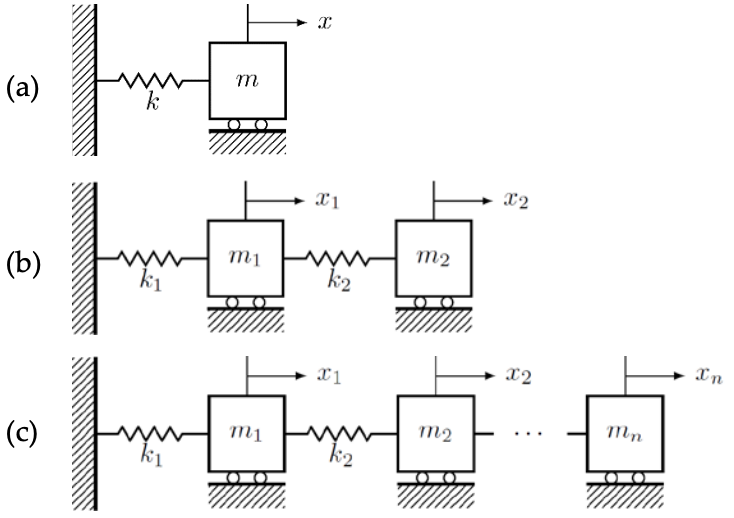
\includegraphics[scale=0.5]{Immagini/GradiDiLibertà.png}
    \caption{Esempi di sistemi vibranti ad uno (a), due (b) ed \textit{n} (c) gradi di libertà.}
    \label{GradiDiLibertà}
\end{figure}
\paragraph{Lineari o Non lineari} Se le equazioni che descrivono il moto del sistema sono lineari, il sistema vibrante si dice \textit{lineare}. Solitamente i sistemi di questo tipo sono quelli per cui l'ampiezza di vibrazione è ridotta, mentre sistemi con ampiezza di vibrazioni rilevanti determinano fenomeni più complessi che vengono descritti da equazioni non lineari. 
\paragraph{Liberi o Forzati} Un sistema non influenzato da alcuna forza esterna, in seguito ad un perturbazione iniziale, vibra in modo \textit{libero}. Se il sistema è soggetto ad una forza dinamica esterna, come una forza armonica generata da una massa rotante, il risultato è un sistema sottoposto a \textit{vibrazione forzata}.
\paragraph{Smorzati o Non smorzati} Lo smorzamento dissipa energia del sistema, causando una diminuzione della vibrazione. Se lo smorzamento è presente all'interno del sistema, la vibrazione risultante sarà chiamata \textit{vibrazione smorzata}. Un certo grado di smorzamento è presente in ogni sistema, tuttavia, se il valore è trascurabile, può non comparire all'interno delle equazioni e il sistema risulta \textit{non smorzato}.
\paragraph{Discreti o Continui} In molti casi il sistema può essere schematizzato assumendo che la massa, la flessibilità e lo smorzamento, siano tutte caratteristiche concentrate all'interno di singoli componenti quali masse, molle e smorzatori. Sistemi di questo tipo vengono definiti sistemi \textit{discreti}. Tuttavia, sono presenti anche sistemi meccanici in cui la massa e la flessibilità sono distribuite in modo continuo (es. travi).
\begin{figure}[h]
    \centering
    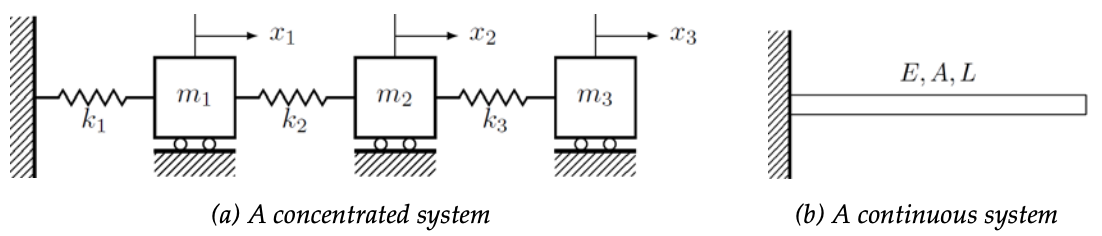
\includegraphics[scale=0.5]{Immagini/DiscretoContinuo.png}
    \caption{Sistema discreto e sistema continuo.}
    \label{DiscretoContinuo}
\end{figure}

Il sistema oggetto di studio è un sistema \textit{discreto}, \textit{lineare}, \textit{forzato}.
\subsection{Componenti del sistema}
\paragraph{Molla} Le molle sono responsabili dell'immagazzinamento di energia potenziale all'interno di un sistema vibrante. In un'analisi ideale, le molle sono assunte senza massa e con un contributo di smorzamento nullo. 
La forza è funzione dello spostamento $F=F(x)$, e si oppone alla direzione dello spostamento applicato. Per molle lineari l'espressione della forza corrisponde a 
\begin{equation}
    F=k \Delta x= k (x_2-x_1)
\end{equation}
\begin{figure}[h]
    \centering
    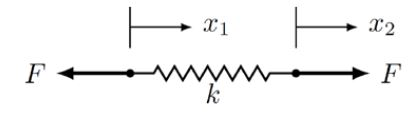
\includegraphics[scale=0.6]{Immagini/MollaLineare.JPG}
    \caption{Molla lineare.}
    \label{MollaLineare}
\end{figure}
\paragraph{Massa} La masse sono responsabili dell'immagazzinamento dell'energia cinetica del sistema. Per semplificare l'analisi, si considera la massa concentrata in un unico punto.
\paragraph{Smorzatore} Lo smorzatore è un meccanismo responsabile della dissipazione di energia all'interno di un sistema vibrante attraverso la conversione in calore, suono o altre forme di energia. Quando è presente smorzamento in un sistema a vibrazione libera, l'ampiezza di vibrazione diminuisce nel tempo. Ciò non è più vero se il sistema è forzato. 
Questo elemento è caratterizzato da una forza di smorzamento $F$ opposta in direzione ma proporzionale alla differenza di velocità relativa tra le due estremità ($\Delta \dot x$). La costante che lega questi due termini è la \textit{costante di smorzamento viscoso} $c$:
\begin{equation}
    F=c \Delta \dot x= c(\dot x_2-\dot x_1)
\end{equation}
\begin{figure}[h]
    \centering
    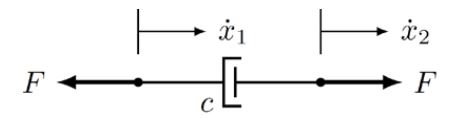
\includegraphics[scale=0.6]{Immagini/SmorzatoreLineare.JPG}
    \caption{Smorzatore lineare.}
    \label{SmorzatoreLineare}
\end{figure}




%Gli assorbitori dinamici sono componenti che si prefiggono lo scopo di ridurre le oscillazioni del sistema. In un’analisi leggermente più approfondita si schematizza con $m_1$ la massa del sistema che subisce la vibrazione e di cui si vuole ridurne l’effetto, mentre con $m_2$ si indica la massa che, accoppiata ad un elemento elastico, costituisce l’assorbitore dinamico. 

%A seconda della configurazione delle masse con cui il sistema viene schematizzato, gli assorbitori dinamici si dividono in  “undamped” oppure “damped” . Nel primo caso (Figura  \ref{sistemanonsmorzato}), le masse $m_1$ e $m_2$ sono collegate tra loro attraverso un solo elemento elastico.

%Nel secondo caso (Figura \ref{sistemasmorzato}) le due masse sono collegate attraverso una molla ed uno smorzatore.

%Uno smorzatore ha come principale obiettivo quello di ridurre drasticamente l’ampiezza dell’oscillazione di un sistema vibrante. Il prezzo da pagare per introdurre un oggetto di questo tipo è la complicazione del modello di sistema, rendendo necessario l’utilizzo di strumenti di calcolo matriciale (es. MATLAB).

%All’aumentare del rateo di smorzamento, l’effetto complessivo sul sistema sarà una riduzione dell’ampiezza di oscillazione del sistema secondario alle due frequenze naturali, ma un aumento dell’ampiezza di oscillazione del sistema primario alla sua frequenza naturale. \\\\
%In conclusione, si avrà sì una riduzione della vibrazione del sistema combinato alle frequenze naturali di funzionamento, ma il sistema primario non raggiungerà mai ampiezza di oscillazione nulla per la propria frequenza naturale. 

